% =============================================================================
%  BAO CAO DO AN CUOI KY, NHOM 8
%  Mon: Chuyen de nghien cuu va Xu ly ngon ngu tu nhien
%
%  QUAN TRONG VE CACH BIEN DICH:
%  Nen chon LuaLaTeX tren Overleaf: Menu > Compiler > LuaLaTeX.
%  Ly do: ma hoa T1 mac dinh cua template ACL khong chua cac ky tu tieng Viet
%  nhu a-grave-breve, u-tilde-horn, o-dot-horn.
%
%  Tu 2026-08-11 file da co khoi \ifPDFTeX nen bien dich bang pdfLaTeX cung
%  ra ban dung (nhanh do nap ma hoa T5 cua vntex). Chi tiet o phan mo dau.
%
%  Can co trong cung thu muc: acl.sty, acl_natbib.bst, custom.bib
%  (lay tu template chinh thuc: https://github.com/acl-org/acl-style-files)
%
%  QUY UOC SOAN THAO: KHONG dung dau gach dai (em dash). Dung dau phay, dau
%  hai cham, hoac ngoac don thay the.
% =============================================================================

\documentclass[11pt]{article}

% Bo [review] khi nop ban chinh thuc co ten tac gia.
\usepackage{acl}

\usepackage{microtype}

% ---------------------------------------------------------------------------
% CHON FONT THEO BO BIEN DICH. Doc ky truoc khi sua.
%
% LOI DA GAP (bien ban 2026-08-11): ban truoc goi thang \babelfont{rm}{...}.
% \babelfont CHI ton tai voi LuaTeX va XeTeX. Khi bien dich bang pdfLaTeX,
% babel khong dung lai ma DAT THONG DIEP LOI VAO TRANG GIAY, tai thoi diem
% \begin{document}. Doan chu la "only-lua-xermTeXGyreTermesX" nhin thay tren
% ban in chinh la thong diep do: ma loi "only-lua-xe" noi lien hai tham so
% "rm" va ten font.
%
% Va vi \maketitle cua acl.sty goi \twocolumn, ma \twocolumn luon ngat sang
% trang moi, nen doan chu loi do chiem tron trang 1 con tieu de bi day xuong
% trang 2. Trang trang o dau bao cao va doan chu la la CUNG MOT LOI.
%
% Khoi \ifPDFTeX duoi day lam file chay duoc voi ca hai bo bien dich, nen
% chon nham compiler khong con sinh ra ban in hong nua. Du vay VAN NEN chon
% LuaLaTeX tren Overleaf (Menu > Compiler > LuaLaTeX) vi nhanh fontspec cho
% chu tieng Viet dep hon.
% ---------------------------------------------------------------------------
\usepackage{iftex}
\ifPDFTeX
  % pdfLaTeX: phai dung ma hoa T5 cua vntex. T1 KHONG chua ky tu tieng Viet.
  % Dat sau \usepackage{acl} nen T5 la ma hoa mac dinh (lenh nap sau thang).
  \usepackage[T5]{fontenc}
  % Times cho nhanh pdfLaTeX (bien ban 2026-09-13). Overleaf cua nhom bien dich
  % bang pdfLaTeX; khong co dong nay thi chu ra Computer Modern, rong hon Times
  % nen phan than dai 9 trang (vuot gioi han 8) va cot trai trang 1 bi day het
  % dung o cuoi tom tat, tieu de muc 1 nhay sang cot phai, TeX gian khoang doc
  % duoi "Tom tat noi dung" thanh 39 pt cho day cot. Voi Times: than 8 trang,
  % khoang do 13,6 pt. vntex co san t5ptm.fd va phong urwvn cho tieng Viet;
  % Times cung la phong chuan cua mau ACL. Da bien dich kiem bang pdfTeX 1.40.29.
  \usepackage{times}
\else
  % LuaLaTeX hoac XeLaTeX. Ba font TeX Gyre di cung mot goi trong TeX Live
  % nen neu thieu thi thieu ca ba; khi do chi can chu thich ca ba dong,
  % Latin Modern mac dinh cung co day du dau tieng Viet.
  \usepackage{fontspec}
  \setmainfont{TeX Gyre Termes}
  \setsansfont{TeX Gyre Heros}
  \setmonofont{TeX Gyre Cursor}
\fi
\usepackage[vietnamese]{babel}

% Tieu de danh muc tai lieu tham khao bang tieng Viet. acl.sty viet cung chu
% "References" ben trong \thebibliography, nen \refname cua babel khong co tac
% dung; phai va lenh do. \patchcmd thay lan xuat hien DAU TIEN, chinh la tieu
% de in ra (hai lan sau nam trong \@mkboth, chi dung cho tieu de chay dau trang
% ma mau ACL khong in). Lenh chua @ nen phai boc \makeatletter. Neu acl.sty tren
% Overleaf khac ban chinh thuc thi va that bai: tieu de giu "References", log co
% canh bao, ban build khong vo.
\usepackage{etoolbox}
\newcommand{\tailieuthamkhao}{Tài liệu tham khảo}
\makeatletter
\patchcmd{\thebibliography}{References}{\tailieuthamkhao}{}{%
  \PackageWarningNoLine{acl_latex}{Khong doi duoc tieu de References}}
\makeatother

\usepackage{graphicx}
\usepackage{booktabs}
\usepackage{amsmath}
\usepackage{amssymb}
\usepackage{xcolor}

% Thu hep khoang cach giua cac cot cua bang. Mac dinh 6pt lam nhieu bang so
% lieu rong hon mot cot cua bo cuc hai cot, khien chung tran sang cot ben canh
% va de len chu. 4pt du thoang ma van vua.
\setlength{\tabcolsep}{4pt}

% Danh dau cho phan chua co so lieu. In do dam mau do de khong the nop nham
% mot ban bao cao con lo trong.
\newcommand{\chuacoso}[1]{\textcolor{red}{\textbf{[CHUA CO SO LIEU: #1]}}}

% KHONG dat \\ trong tieu de. Tieu de dai hon mot dong nen dau ngat tay roi
% vao giua dong, de lai mot dong chi co hai chu "hai," va mot dong chi co
% "corpus". De LaTeX tu ngat thi ba dong can nhau.
\title{Hyena cho tiếng Việt: Mô hình ngôn ngữ tích chập dài dưới bậc hai,
phân tích ablation và khởi tạo bộ lọc từ cấu trúc thông tin của corpus}

% Ban truoc dung \And de xep ba tac gia thanh ba cot canh nhau. Moi dia chi
% thu dien tu dai 25 ky tu, ba dia chi canh nhau vuot chieu ngang trang nen
% chung dinh lien vao nhau khong con khoang trong. Ca nhom cung mot don vi
% nen gop lam mot khoi va viet chung ten mien, dung cach thong dung cua ACL.
% Ma so hoc vien khong mat di vi no chinh la phan dau dia chi thu.
\author{
  Nguyễn Cao Trung Kiên \quad Tô Huỳnh Minh Tiến \quad Trần Tú Quang \\
  Trường Đại học Công nghệ Thông tin, ĐHQG-HCM \\
  \texttt{\{250201069, 250201095, 250201084\}@grad.uit.edu.vn}
}

\begin{document}
\maketitle

\begin{abstract}
Toán tử Hyena \citep{poli2023hyena} thay thế self-attention bằng đệ quy đan xen
tích chập dài tham số hoá ngầm và cổng nhân điều khiển bởi dữ liệu, cho chi phí
dưới bậc hai theo độ dài chuỗi; mọi thực nghiệm ngôn ngữ của bài báo gốc đều
trên tiếng Anh. Chúng tôi cài đặt lại Hyena kèm bộ kiểm thử tính nhân quả, áp
dụng cho mô hình ngôn ngữ tiếng Việt với nhánh đối chứng tiếng Anh, và đề xuất
khởi tạo phân bố suy giảm của bộ lọc từ đường cong thông tin tương hỗ đo trên
corpus. Ở khoảng 7,5 triệu tham số, cùng 50 triệu token và cùng siêu tham số,
Hyena có perplexity thấp hơn Transformer 19,5\% trên tiếng Việt và 14,7\% trên
tiếng Anh, nhưng ưu thế này không chuyển thành ưu thế phân loại trên UIT-VSFC.
Tiếng Việt mang thông tin tương hỗ cục bộ gấp 1,7 đến 2,3 lần
tiếng Anh ở khoảng cách ngắn. Trên tiếng Việt, đặt phân bố suy giảm theo một
nguyên tắc, cách đều theo thang log hoặc suy từ corpus, giảm khoảng 0,9 PPL so
với một khoảng chọn tuỳ ý; trên tiếng Anh hiệu ứng cùng chiều nhưng không qua
hiệu chỉnh so sánh bội. Khởi tạo từ corpus không vượt được đường cơ sở thang
log một cách có ý nghĩa. Trên nhánh tiếng Anh, dùng $\alpha$ suy từ tiếng Việt
không làm perplexity tăng có ý nghĩa thống kê ($p = 0{,}28$); chiều hoán đổi
ngược lại chưa được kiểm tra.
\end{abstract}

% =============================================================================
\section{Giới thiệu}
% =============================================================================

Cơ chế self-attention \citep{vaswani2017attention} có chi phí tính toán và bộ
nhớ tăng theo bình phương độ dài chuỗi, đặt ra giới hạn cứng cho lượng ngữ cảnh
mà mô hình có thể xử lý. Nhiều hướng nghiên cứu tìm cách vượt qua giới hạn này,
trong đó các mô hình không gian trạng thái \citep{gu2021s4, mehta2022gss,
dao2023h3} và tích chập dài trở thành những phương án thay thế đáng chú ý.

Hyena \citep{poli2023hyena} là một trong những kiến trúc đầu tiên không dùng
attention dày đặc mà vẫn đạt chất lượng tương đương Transformer trên mô hình
hoá ngôn ngữ ở quy mô lớn. Toán tử này đan xen tích chập dài tham số hoá ngầm
với cổng nhân điều khiển bởi dữ liệu, cho chi phí $O(N L \log_2 L)$ thay vì
$O(L^2)$. Dòng nghiên cứu này về sau dẫn tới các kiến trúc chọn lọc trạng thái
như Mamba \citep{gu2023mamba}.

Toàn bộ thực nghiệm ngôn ngữ trong bài báo gốc thực hiện trên tiếng Anh, cụ thể
là WikiText103 \citep{merity2017pointer} và The Pile \citep{gao2020pile}. Chưa
có bằng chứng nào về hành vi của Hyena trên tiếng Việt, một ngôn ngữ có đặc
điểm chữ viết khác hẳn: chữ Quốc ngữ tách rời theo âm tiết, nên một từ ghép
nhiều âm tiết bị tách thành nhiều token khi token hoá theo khoảng trắng. Các mô
hình ngôn ngữ tiếng Việt hiện có phần lớn dựa trên kiến trúc Transformer
\citep{nguyen2020phobert}.

Báo cáo này có ba đóng góp.

Thứ nhất, chúng tôi cài đặt lại toán tử Hyena bám sát đặc tả gốc và
\emph{kiểm chứng} tính nhân quả của cài đặt bằng bộ kiểm thử tự động, trong đó
có phép kiểm dựa trên gradient kèm một phép kiểm ngược cố ý cài lỗi.
Thứ hai, chúng tôi đo đường cong suy giảm thông tin tương hỗ trên corpus tiếng
Việt và tiếng Anh, dùng nó để khởi tạo phân bố suy giảm của bộ lọc Hyena thay
cho việc đặt tham số này bằng trực giác. Thứ ba, chúng tôi báo cáo đầy đủ các
kết quả không ủng hộ giả thuyết ban đầu của chính mình: khởi tạo từ corpus không
vượt được một đường cơ sở không dùng thông tin ngôn ngữ, và mức độ đặc thù ngôn
ngữ của bộ lọc phụ thuộc vào quy ước ánh xạ nhiều hơn chúng tôi dự kiến.

% =============================================================================
\section{Nền tảng: toán tử Hyena}
% =============================================================================

\subsection{Định nghĩa}

Gọi $u \in \mathbb{R}^{L \times D}$ là chuỗi đầu vào. Hyena bậc $N$ trước hết
tính $N+1$ phép chiếu tuyến tính của đầu vào, tiếp theo là một tích chập ngắn
theo kênh, thu được $(x^1, \dots, x^N, v)$. Toán tử được định nghĩa bằng đệ quy
(Định nghĩa 3.1 trong \citealp{poli2023hyena}):
\begin{align}
z^1_t &= v_t \nonumber\\
z^{n+1}_t &= x^n_t \cdot (h^n \ast z^n)_t, \quad n = 1 \dots N \label{eq:hyena}\\
y_t &= z^{N+1}_t \nonumber
\end{align}
trong đó $\ast$ là tích chập nhân quả dài và $h^n$ là các bộ lọc học được. Mỗi
tích chập được tính trong miền Fourier, cho độ phức tạp tổng cộng
$O(N L \log_2 L)$.

Bài báo gốc chỉ ra rằng Hyena bậc 1 tương ứng với GSS \citep{mehta2022gss} và
bậc 2 tương ứng với H3 \citep{dao2023h3}, nên bậc $N$ là một trục thiết kế có
ý nghĩa chứ không phải một tham số tuỳ ý.

\subsection{Bộ lọc tham số hoá ngầm}

Yếu tố cho phép bộ lọc có độ dài lớn mà số tham số không tăng theo $L$ là cách
tham số hoá ngầm:
\begin{equation}
h_t = \mathrm{Window}(t) \cdot (\mathrm{FFN} \circ \mathrm{PositionalEncoding})(t)
\label{eq:filter}
\end{equation}
với $\mathrm{Window}(t) = \exp\{-\alpha t\} + b$, trong đó $\alpha$ thay đổi theo
từng kênh nhằm buộc các bộ lọc có độ dài khác nhau, còn $b$ là độ lệch học được
để bộ lọc không bị triệt tiêu về 0 sau độ dài do $\alpha$ quy định (bài báo gốc cũng
thêm số hạng này). Mạng $\mathrm{FFN}$ dùng kích
hoạt tuần hoàn tần số cao (sine), theo dòng biểu diễn ngầm
\citep{sitzmann2020siren, romero2021ckconv}, để khắc phục thiên lệch tần số thấp
của mạng nơ-ron. Tính nhân quả được bảo đảm bằng cách đánh giá bộ lọc tại
$t = 0 \dots L-1$ rồi đệm 0 cả tín hiệu lẫn bộ lọc tới độ dài ít nhất $2L-1$
trước khi biến đổi Fourier.

Phân bố $\{\alpha_i\}$ được mô tả là ``thay đổi theo kênh'' nhưng bài báo gốc không
quy định khoảng giá trị cụ thể, cũng không gắn nó với thống kê của ngôn ngữ
đích. Đây là khoảng trống mà đóng góp của chúng tôi hướng tới.

% =============================================================================
\section{Khởi tạo bộ lọc từ cấu trúc thông tin của corpus}
% =============================================================================

\subsection{Động cơ}

Với $t$ chuẩn hoá về $[0,1]$ trên $L$ vị trí, kênh thứ $i$ suy giảm còn $1/e$
tại token thứ khoảng $L/\alpha_i$. Chúng tôi gọi đại lượng này là \emph{độ dài
hiệu dụng} của kênh. Câu hỏi nghiên cứu là: nếu tập độ dài hiệu dụng được đặt
tương ứng với vùng khoảng cách chứa thông tin dự đoán trong corpus, mô hình có
sử dụng ngân sách kênh hiệu quả hơn không?

\subsection{Đại lượng đo và lý do không dùng bộ tách từ}

Một phương án trực tiếp là dùng bộ tách từ tiếng Việt để lấy phân bố số âm tiết
mỗi từ. Chúng tôi không chọn phương án này vì nó làm mất tính so sánh của nhánh
đối chứng: tiếng Anh không có bộ tách từ tương đương, nên mọi khác biệt quan sát
được đều có thể quy cho công cụ đo thay vì cho ngôn ngữ.

Thay vào đó chúng tôi đo trực tiếp thông tin tương hỗ giữa hai token cách nhau
$d$ vị trí:
\begin{equation}
I(d) = \sum_{x,y} p_d(x,y) \log \frac{p_d(x,y)}{p(x)\,p(y)}
\label{eq:mi}
\end{equation}
Hai ngôn ngữ được đo bằng cùng công thức và cùng quy trình ước lượng.
\citet{lin2017critical} đã khảo sát sự suy giảm của đại lượng này trong văn bản
tự nhiên; chúng tôi dùng nó cho một mục đích khác là khởi tạo bộ lọc.

\subsection{Xử lý độ chệch của ước lượng}

Ước lượng hợp lý cực đại của thông tin tương hỗ luôn chệch dương trên mẫu hữu
hạn \citep{paninski2003estimation}, và độ chệch tăng theo bình phương cỡ bảng chữ cái; bỏ qua điều này sẽ dẫn
tới kết luận rằng ngôn ngữ có corpus nhỏ hơn mang nhiều thông tin tầm xa hơn.
Chúng tôi khử độ chệch bằng cách trừ đường nền xáo trộn: hoán vị ngẫu nhiên corpus
phá vỡ mọi phụ thuộc giữa các vị trí, nên thông tin tương hỗ đo trên bản hoán vị
chính là độ chệch. Ngoài ra chúng tôi thô hoá bảng chữ cái xuống $K$ ký hiệu thường gặp
nhất, làm giảm độ chệch theo $K^2$; việc thô hoá khiến ước lượng thiên về thận trọng.

\subsection{Hiệu chuẩn công cụ đo}

Một công cụ đo chưa được hiệu chuẩn trên dữ liệu có đáp án biết trước thì chưa
đủ căn cứ để rút ra kết luận. Chúng tôi kiểm tra công cụ đo trên bốn chuỗi nhân
tạo. Trên chuỗi độc lập hoàn toàn, đáp án đúng là $I = 0$ và kết quả đo còn dư
2,82\% độ chệch. Trên chuỗi sao chép chu kỳ $k = 8$, đỉnh xuất hiện đúng tại
$d = 8$ và cao gấp 84 lần mức nền. Trên chuỗi Markov, công cụ cho $I(1) = 2{,}79$,
giảm đơn điệu và gần như triệt tiêu tại $d = 64$. Trên chuỗi suy biến toàn 0,
công cụ báo lỗi và không sinh $\alpha$ thay vì trả về một phân bố vô nghĩa.

\subsection{Ánh xạ sang phân bố suy giảm}

Chúng tôi coi $I(d)$ là khối lượng thông tin nằm tại khoảng cách $d$, chuẩn hoá
thành một phân bố xác suất trên khoảng cách, rồi lấy $D$ phân vị cách đều làm
tập độ dài hiệu dụng $\{\ell_i\}$, cuối cùng đặt $\alpha_i = L / \ell_i$. Vùng
khoảng cách tập trung nhiều thông tin sẽ được phân bổ nhiều kênh hơn.

Trong các lần chạy khởi tạo từ corpus (mục~\ref{sec:e4text}), tệp $\alpha$ được
sinh từ phép đo BPE với $K=500$, nhưng mô hình ngôn ngữ chính lại huấn luyện với
đơn vị âm tiết, nên độ dài hiệu dụng được áp dụng nguyên vẹn từ đơn vị token BPE
sang vị trí token âm tiết.
Tỉ lệ ký tự trên mỗi token trong file đo là 3,851 so với 4,118 ở nhánh tiếng
Việt và 4,155 so với 5,100 ở nhánh tiếng Anh, tức lệch thang khoảng 6,5\% và
18,5\%. Chúng tôi xem đây là hạn chế về diễn giải, không quy trực tiếp thành sai
số perplexity vì chưa có thí nghiệm cô lập yếu tố này.

\subsection{Hai đường cơ sở, và vì sao cần cả hai}

Chúng tôi so sánh với hai đường cơ sở. Đường thứ nhất, ký hiệu \textsf{uniform},
đặt $\alpha$ cách đều tuyến tính trong một khoảng do chúng tôi chọn. Đường thứ
hai, ký hiệu \textsf{logspace}, đặt độ dài hiệu dụng cách đều theo thang log từ
1 tới $L$.

Đường cơ sở \textsf{logspace} cần thiết vì lý do sau. Phép đo cho thấy 80\%
tới 90\% thông tin nằm trong khoảng cách 34 token, tuỳ ngôn ngữ và bộ token
hoá, trong khi cấu hình \textsf{uniform}
đặt \emph{toàn bộ} 256 kênh ra xa hơn 64 token (Bảng~\ref{tab:dodaihieudung}).
So sánh đề xuất với một cấu hình lệch xa như vậy là so sánh với một đường cơ sở
yếu: vượt được nó không chứng minh giá trị của đề xuất. Mọi kết luận về đề xuất
trong báo cáo này đều rút ra từ so sánh với \textsf{logspace}.

% =============================================================================
\section{Thiết lập thí nghiệm}
% =============================================================================

\subsection{Nguyên tắc so sánh công bằng}

Trong so sánh chính giữa Hyena và Transformer, mọi cấu hình chỉ khác nhau ở
toán tử trộn token. Embedding, pre-LayerNorm, khối MLP, kết nối residual,
weight tying, cách khởi tạo và lịch learning rate giữ nguyên vẹn như nhau.
Riêng các nhánh ablation thay đổi cấu trúc bên trong toán tử nên
không giữ nguyên tổng tham số: bậc $N = 1$ ít hơn cấu hình chuẩn 4,4\%, bậc
$N = 3$ nhiều hơn 4,4\%, bỏ positional embedding ít hơn 1,7\% (xem
Bảng~\ref{tab:e3}).

Chúng tôi dùng positional embedding học được cho cả hai loại mô hình: attention
bắt buộc cần thông tin vị trí còn Hyena thì không, nên dùng cho một bên mà không
dùng cho bên kia sẽ tạo ra hai biến thay đổi thay vì một; một nhánh ablation
riêng kiểm tra Hyena có thật sự không cần. Huấn luyện tính theo ngân sách token
cố định chứ không theo số epoch, vì so theo epoch sẽ thiên vị mô hình chạy nhanh
hơn.

\subsection{Mô hình và dữ liệu}

Mô hình 4 lớp, $d_{\text{model}} = 256$, 8 đầu attention, $d_{\text{ff}} = 1024$,
$L = 512$, từ điển 16k. Số tham số đo được: Hyena 7.553.280 và Transformer
7.383.552, lệch 2,30\%.

Dữ liệu lấy từ Wikipedia tiếng Việt và tiếng Anh (bản \texttt{20231101}).
Nhánh tiếng Anh được lấy mẫu 110.000 tài liệu rồi cắt xuống đúng 38.250.964
token của nhánh tiếng Việt, nên hai nhánh có cùng số token huấn luyện duy nhất.
Cả hai sau đó huấn luyện trên cùng 49.995.776 token, tức cùng 6.103 bước và
cùng khoảng 1,31 epoch.

Chúng tôi khảo sát hai đơn vị token hoá: âm tiết, tức tách theo khoảng trắng, vốn
là đơn vị tự nhiên của chữ Quốc ngữ; và BPE \citep{sennrich2016bpe} mức byte
\citep{radford2019gpt2}, huấn luyện trên chính corpus, không sinh token ngoài từ
điển. Với tiếng Anh, tách theo khoảng trắng cho ra đơn vị từ chứ không phải âm
tiết, nên nhánh đối chứng phải được diễn giải tương ứng.

\subsection{Kiểm chứng tính đúng đắn của cài đặt}

Một mô hình ngôn ngữ nhân quả bị cài đặt sai, để rò rỉ thông tin từ các vị trí
tương lai, vẫn huấn luyện bình thường và cho perplexity thấp bất thường. Đây là
loại lỗi khó phát hiện và nguy hiểm nhất trong dạng nghiên cứu này. Chúng tôi
loại trừ lỗi này bằng bộ kiểm thử tự động, trong đó phép kiểm cốt lõi dùng
gradient: lấy đạo hàm của đầu ra tại vị trí $t$ theo đầu vào tại mọi vị trí
$s > t$ và yêu cầu kết quả bằng 0. Attention cho giá trị đúng bằng 0 nhờ mặt nạ nhân quả;
Hyena đạt dưới $10^{-15}$ trên mọi biến thể đã kiểm (lần chạy khi viết báo cáo
này cho $3{,}8 \times 10^{-16}$), tức nhân quả tới sai số làm tròn của phép biến
đổi Fourier thuận và nghịch. Quan trọng hơn, chúng tôi bổ sung một \emph{phép kiểm ngược}: chủ động đưa vào
một lỗi nhân quả điển hình (cắt lệch phần đệm của tích chập ngắn) và xác nhận tỉ
lệ rò rỉ tăng lên khoảng $2$. Chênh lệch hơn 15 bậc độ lớn cho thấy bộ kiểm thử
thực sự có khả năng phát hiện lỗi, chứ không cho kết quả đạt chỉ vì thiếu độ
nhạy.

% =============================================================================
\section{Kết quả}
% =============================================================================

\subsection{Cấu trúc thông tin của tiếng Việt so với tiếng Anh}

Bảng~\ref{tab:mi} trình bày tỉ lệ $I_{\text{vi}}(d) / I_{\text{en}}(d)$ đo với
hai cách token hoá. Cột thứ nhất dùng token hoá theo âm tiết với từ điển 16k;
cột thứ hai dùng BPE mức byte, không sinh token ngoài từ điển, với đúng
10.000.000 token cho mỗi ngôn ngữ.

\begin{table}[t]
\centering
\small
\begin{tabular}{rrr}
\toprule
$d$ & âm tiết & BPE (0\% OOV) \\
\midrule
1   & 1,71 & 1,66 \\
6   & 1,66 & 2,27 \\
13  & 1,56 & 1,94 \\
34  & 1,26 & 1,55 \\
88  & 0,94 & 1,27 \\
167 & (dưới nhiễu) & 1,03 \\
\bottomrule
\end{tabular}
\caption{Tỉ lệ thông tin tương hỗ giữa tiếng Việt và tiếng Anh theo khoảng
cách. Cột âm tiết có nhiễu loạn do tỉ lệ token ngoài từ điển chênh lệch
(tiếng Anh 10,26\% so với tiếng Việt 2,59\%); cột BPE khử nhiễu loạn này.}
\label{tab:mi}
\end{table}

\begin{figure*}[t]
\centering
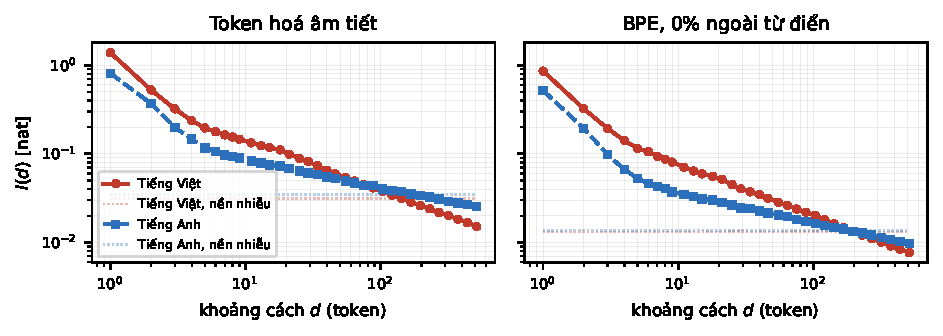
\includegraphics[width=\textwidth]{figures/fig_mi_decay.pdf}
\caption{Suy giảm thông tin tương hỗ theo khoảng cách. Đường chấm mảnh là nền
nhiễu ước lượng; phần đường cong nằm dưới nó không mang thông tin. Với token
hoá âm tiết (trái), hai đường cắt nhau quanh $d \approx 88$; khi khử token
ngoài từ điển bằng BPE (phải), điểm cắt biến mất và tiếng Việt nằm trên tiếng
Anh trong toàn vùng tín hiệu nằm trên nền nhiễu.}
\label{fig:mi}
\end{figure*}

Ba nhận xét.

Thứ nhất, với phép đo BPE, tiếng Việt mang nhiều thông tin tương hỗ cục bộ hơn
tiếng Anh ở mọi khoảng cách trong vùng đo được, nhưng ưu thế tập trung ở khoảng
cách ngắn: tỉ lệ đạt 1,66 tới 2,27 ở $d \le 13$ rồi giảm dần về 1,03 ở $d = 167$
(Bảng~\ref{tab:mi}, Hình~\ref{fig:mi}). Với phép đo âm tiết, ưu thế đảo chiều từ
$d \approx 88$, nên phát biểu này chỉ vững với phép đo BPE.

Thứ hai, phép đo bằng âm tiết cho thấy hai đường cắt nhau tại $d \approx 88$,
nhưng điểm cắt này \emph{biến mất} khi khử token ngoài từ điển. Đây là sai lệch
do phương pháp đo: mọi từ hiếm của tiếng Anh bị gộp vào một ký hiệu duy nhất,
làm mất thông tin của tiếng Anh một cách hệ thống. Chúng tôi nêu điểm này như
một cảnh báo: nếu chỉ đo bằng âm tiết, chúng tôi đã rút ra kết luận sai.

Thứ ba, tín hiệu giảm xuống dưới mức nhiễu ở $d > 121$ với phép đo âm tiết và
$d > 167$ với BPE. Mọi phát biểu về khoảng cách xa hơn các mốc này đều không có
căn cứ.

\subsection{Phân bố kênh bộ lọc}

Bảng~\ref{tab:dodaihieudung} so sánh phân bố độ dài hiệu dụng của bốn cấu hình.

\begin{table}[t]
\centering
\small
\begin{tabular}{lrrr}
\toprule
Cấu hình & $\le 4$ & $\le 34$ & trung vị \\
\midrule
\textsf{uniform} & 0 & 0 & 169,3 \\
\textsf{logspace} & 57 & 145 & 22,6 \\
corpus, tiếng Việt & 142 & 227 & 2,95 \\
corpus, tiếng Anh & 141 & 214 & 2,85 \\
\bottomrule
\end{tabular}
\caption{Số kênh trên tổng 256 có độ dài hiệu dụng dưới ngưỡng cho trước
($L = 512$). Ngưỡng 34 token là nơi chứa 87,5\% thông tin với tiếng Việt và
79,9\% với tiếng Anh khi đo bằng âm tiết, 88,7\% và 83,5\% khi đo bằng BPE.}
\label{tab:dodaihieudung}
\end{table}


\subsection{Nhánh đối chứng tiếng Anh và độ vững của kết luận}
\label{sec:doichung}

Giả thuyết ban đầu của chúng tôi là bộ lọc suy từ corpus mang tính đặc thù tiếng
Việt. Theo quy ước ánh xạ dùng khi huấn luyện, bộ lọc suy từ corpus tiếng Việt
và tiếng Anh gần nhau: trung vị độ dài hiệu dụng 2,95 so với 2,85 token; trên 256
kênh đã sắp theo phân vị, độ lệch tương đối trung bình
$\mathrm{mean}(|\ell_{\text{vi}}-\ell_{\text{en}}|/\ell_{\text{en}})$ là 14,3\%
(22,3\% nếu lấy $\ell_{\text{vi}}$ làm mẫu số, 17,3\% với thước đo đối xứng),
trong khi bộ lọc tiếng Việt lệch 75,8\% so với \textsf{logspace}. Tăng $K$ từ
500 lên 1000 cho 12,9\%. Tương quan Pearson giữa các log độ dài không phân biệt
được hai trường hợp (0,9974 với cặp Việt và Anh, 0,9377 với cặp Việt và
\textsf{logspace}) vì mọi vector phân vị đều đơn điệu, nên chúng tôi không dùng
nó làm bằng chứng.

Tuy nhiên kết quả này phụ thuộc một quy ước. Hàm \texttt{alphas\_from\_mi} coi
mỗi điểm trên lưới log của $d$ là một khối lượng xác suất mà không nhân với bề
rộng ô quanh điểm đó; lưới log dày ở khoảng cách ngắn nên phân bố bị kéo về các
lag nhỏ. Khi nhân bề rộng ô, trung vị thành 90,5 token với tiếng Việt và 160,5
với tiếng Anh, độ lệch tương đối tăng lên 36,2\% (81,1\% và 48,9\% theo hai
thước đo còn lại), còn độ lệch so với \textsf{logspace} là 163,3\%. Hai bộ lọc
vẫn gần nhau hơn so với đường cơ sở, nhưng không còn gần như trùng nhau, và bộ
lọc tiếng Việt ngắn hơn, cùng chiều với việc tiếng Việt có nhiều thông tin tương
hỗ cục bộ hơn. Vì vậy phân tích hình dạng bộ lọc \emph{không} đủ để bác bỏ tính
đặc thù ngôn ngữ.

Phép thử ở mức huấn luyện là hoán đổi $\alpha$: mô hình tiếng Anh dùng $\alpha$
suy từ tiếng Việt (cùng corpus, cùng cấu hình, 3 seed) đạt 54,77 PPL so với 54,91
khi dùng $\alpha$ của chính nó ($\Delta = -0{,}15$; KTC 95\% [$-0{,}48$; $0{,}18$];
Welch $p = 0{,}28$). Vì perplexity ít nhạy với $\alpha$ (mục~\ref{sec:e4text}),
kết luận có thể rút ra chỉ là: trên tiếng Anh, $\alpha$ suy từ tiếng Việt thay thế
được $\alpha$ của chính mô hình, chứ không phải hai bộ lọc giống nhau; chiều ngược
lại chưa được kiểm tra trên đúng corpus. Đối chứng chạy lại trong cùng phiên cho
perplexity trùng khớp đến từng chữ số với lần chạy gốc ở môi trường khác, nên
chênh lệch không do môi trường gây ra. Các số được tái sinh bởi \texttt{python -m hyena\_study.analyze}.

\subsection{Perplexity trên mô hình ngôn ngữ}

\begin{table}[t]
\centering
% Ban build 2026-08-18 16:19: bang nay o cot trai chay den x = 297,9 pt, tuc
% tran 6,9 pt vao khoang giua hai cot. Siet tabcolsep cho vua.
\setlength{\tabcolsep}{2pt}
\small
\begin{tabular}{llrr}
\toprule
Ngôn ngữ & Mô hình & PPL & KTC 95\% \\
\midrule
Tiếng Việt & Hyena       & \textbf{51,38} $\pm$ 0,13 & [51,05; 51,71] \\
           & Transformer & 63,86 $\pm$ 0,29 & [63,14; 64,58] \\
\midrule
Tiếng Anh  & Hyena       & \textbf{55,82} $\pm$ 0,35 & [54,96; 56,68] \\
           & Transformer & 65,43 $\pm$ 0,18 & [64,99; 65,87] \\
\bottomrule
\end{tabular}
\caption{Perplexity trên tập kiểm tra, 3 seed cho mỗi cấu hình; $\pm$ là độ
lệch chuẩn mẫu. Khoảng tin cậy 95\% theo phân phối $t$ ($t = 4{,}303$).}
\label{tab:e1}
\end{table}

Hyena có perplexity thấp hơn Transformer 19,5\% trên tiếng Việt và 14,7\% trên
tiếng Anh (Bảng~\ref{tab:e1}; Welch, $p < 10^{-4}$ ở cả hai).

Bài báo gốc chỉ khẳng định Hyena \emph{tương đương} Transformer ở quy mô 125 đến
355 triệu tham số; kết quả này thuộc chế độ khác nên không mâu thuẫn, nhưng cần
được diễn giải thận trọng vì hai lý do. Thứ nhất, cả hai kiến trúc dùng chung
learning rate và lịch huấn luyện; bài báo gốc cũng làm vậy nhưng ghi nhận Hyena hưởng lợi từ learning rate
thấp hơn đôi chút. Thứ hai, Transformer chạy nhanh hơn 1,51 lần mỗi token
(mục~\ref{sec:hieunang}), nên ở cùng thời gian thực nó xử lý được nhiều token
hơn. Phát biểu chính xác là ``Hyena vượt Transformer ở cùng số token, cùng siêu tham
số và cùng quy mô này''. Khoảng cách trên tiếng Việt lớn hơn trên tiếng Anh,
nhưng hai corpus khác nhau và tỉ lệ token ngoài từ điển chênh lệch (3,1\% so với
10,5\%), nên chúng tôi không diễn giải chênh lệch này.

\subsection{Ảnh hưởng của đơn vị token hoá}

Ở cùng lượng ký tự, tiếng Việt sinh nhiều token hơn: trên chính corpus huấn
luyện, 4,118 ký tự trên mỗi token so với 5,100 của tiếng Anh, tỉ lệ 1,239.

Chỉ xét tiếng Việt, với token hoá âm tiết Hyena đạt 51,38 so với 63,86 của
Transformer, tỉ lệ 1,243; với BPE là 80,02 so với 96,22, tỉ lệ 1,202 (3 seed mỗi
ô). Cần tránh một sai lầm diễn giải ở đây: perplexity \emph{không so sánh được giữa hai
bộ token hoá khác nhau} vì từ điển khác nhau cho entropy trên mỗi token khác
nhau, nên 51,38 với âm tiết và 80,02 với BPE \emph{không} có nghĩa là âm tiết tốt
hơn. Đại lượng so sánh được là chênh lệch log-loss giữa hai mô hình quy về mỗi ký
tự: Hyena hơn Transformer 0,053 nat/ký tự với âm tiết và 0,048 nat/ký tự với
BPE, cùng chiều và gần nhau. Chúng tôi không ước lượng khoảng tin cậy cho hiệu
của hai con số nên không kết luận đơn vị token hoá làm thay đổi lợi thế của
Hyena. Cũng lưu ý rằng ở $L = 512$ cố định, hai mô hình xử lý cùng số token, nên
tính dưới bậc hai của Hyena không phải là cơ chế giải thích ở đây.

\subsection{Ablation các thành phần của Hyena}

\begin{table}[t]
\centering
\footnotesize
% Do tren ban build 2026-08-18 16:19: bang nay chay den x = 543,7 pt trong khi
% cot chu ket thuc o x = 526 pt, tuc tran 17,7 pt ra le giay. Siet tabcolsep va
% rut tieu de cot cuoi; chi doi chieu rong nen khong doi so trang.
\setlength{\tabcolsep}{2pt}
\begin{tabular}{lrrcr}
\toprule
Cấu hình & PPL & $\Delta$ & KTC 95\% & $p_{\text{Holm}}$ \\
\midrule
Chuẩn (bậc 2, đủ) & 51,38 & & [51,05; 51,71] & \\
\midrule
Bỏ cửa sổ suy giảm & 53,30 & $+1{,}92$ & [52,24; 54,35] & 0,006 \\
Bậc $N = 1$        & 53,11 & $+1{,}73$ & [51,72; 54,49] & 0,024 \\
Bỏ kích hoạt sine  & 51,80 & $+0{,}42$ & [51,49; 52,10] & 0,047 \\
Bậc $N = 3$        & 51,63 & $+0{,}25$ & [49,51; 53,76] & 0,345 \\
Bỏ positional emb  & 50,79 & $-0{,}59$ & [50,14; 51,45] & 0,024 \\
\bottomrule
\end{tabular}
\caption{Ablation trên tiếng Việt, 2 seed mỗi nhánh (cấu hình chuẩn: 3 seed,
khoảng $\alpha$ do chúng tôi chọn). KTC 95\% theo phân phối $t$. $p_{\text{Holm}}$:
Welch hai mẫu so với cấu hình chuẩn, hiệu chỉnh Holm cho 5 phép so sánh. Với 2
seed, bậc tự do Welch chỉ 1,4 đến 3,0 nên mọi kết luận ở bảng này là sơ bộ.}
\label{tab:e3}
\end{table}

Từ mục này, mọi so sánh perplexity dùng kiểm định Welch hai mẫu, hiệu chỉnh Holm
trong từng họ so sánh ở mức 0,05; khoảng tin cậy trong bảng chỉ để mô tả.

Bỏ cửa sổ suy giảm làm perplexity tăng nhiều nhất (+1,92 PPL), xác nhận vai trò của số
hạng $\mathrm{Window}(t)$ trong công thức~\eqref{eq:filter}. Hạ bậc xuống $N=1$
cũng làm perplexity tăng (+1,73), phù hợp với việc H3, tức Hyena bậc 2, được đề xuất
chính vì GSS, tức bậc 1, yếu ở associative recall; nhưng bậc 1 cũng mất 331.776
tham số (4,4\%), nên mức tăng này gộp lẫn hai nguyên nhân mà thiết kế hiện tại
không tách được. Bỏ kích hoạt sine làm perplexity tăng ít (+0,42) và chỉ vừa
đạt ngưỡng ý nghĩa. Bỏ positional embedding lại cho perplexity \emph{thấp hơn} 0,59, phù hợp
với lập luận rằng bộ lọc tích chập đã mang thông tin vị trí. Bậc $N=3$ không
khác biệt. Vì bậc tự do Welch rất nhỏ, chúng tôi coi các kết luận này là sơ bộ.

\subsection{Khởi tạo bộ lọc từ corpus}
\label{sec:e4text}

\begin{table}[t]
\centering
\small
\begin{tabular}{llrr}
\toprule
Ngôn ngữ & Khởi tạo & PPL & KTC 95\% \\
\midrule
Tiếng Việt & \textsf{uniform}  & 51,38 & [51,05; 51,71] \\
           & \textsf{logspace} & 50,48 & [50,33; 50,62] \\
           & corpus            & \textbf{50,19} & [49,93; 50,45] \\
\midrule
Tiếng Anh  & \textsf{uniform}  & 55,82 & [54,96; 56,68] \\
           & \textsf{logspace} & 54,97 & [54,56; 55,37] \\
           & corpus            & \textbf{54,91} & [54,53; 55,29] \\
\bottomrule
\end{tabular}
\caption{Ảnh hưởng của cách khởi tạo phân bố suy giảm, 3 seed cho mỗi ô.}
\label{tab:e4}
\end{table}

Bảng~\ref{tab:e4} được kiểm bằng Welch với hiệu chỉnh Holm cho sáu phép so sánh
cặp.

Trên tiếng Việt, cả \textsf{logspace} lẫn corpus đều vượt \textsf{uniform}, lần
lượt 0,90 và 1,19 PPL ($p_{\text{Holm}} = 0{,}012$ và $0{,}002$). Trên tiếng Anh
hiệu ứng cùng chiều và cùng độ lớn, 0,85 và 0,90 PPL, nhưng không qua hiệu chỉnh
($p = 0{,}034$ và $0{,}030$ trước hiệu chỉnh; $p_{\text{Holm}} = 0{,}097$). Như
vậy khoảng giá trị của $\alpha$ có ảnh hưởng đo được trên tiếng Việt, còn trên
tiếng Anh mới dừng ở mức gợi ý.

Corpus hơn \textsf{logspace} 0,285 PPL trên tiếng Việt ($p = 0{,}024$ trước hiệu
chỉnh, $p_{\text{Holm}} = 0{,}097$) và 0,05 PPL trên tiếng Anh ($p = 0{,}70$).
Chúng tôi không có căn cứ kết luận rằng suy phân bố suy giảm từ corpus tốt hơn
cách đều theo thang log. Điều ngược lại cũng chưa được chứng minh: trên tiếng
Việt, khoảng tin cậy 95\% chưa hiệu chỉnh của hiệu là [0,07; 0,50] PPL.

Kết quả này còn cho thấy một giới hạn của thiết kế. Bộ lọc corpus lệch
\textsf{logspace} 75,8\% mà perplexity chỉ khác 0,05 đến 0,29, tức perplexity ở
quy mô này ít nhạy với phân bố $\alpha$ trong một vùng hợp lý. Một cơ chế khả dĩ,
chưa kiểm chứng, là độ lệch $b$ của cửa sổ và mạng FFN sinh bộ lọc bù lại một
phần khởi tạo trong khi huấn luyện. Vì vậy thí nghiệm này không đủ độ nhạy để trả lời câu
hỏi bộ lọc có đặc thù ngôn ngữ hay không, và việc phần chênh lệch nhỏ xuất hiện
trên cả hai ngôn ngữ không phải là bằng chứng cho điều đó.

\subsection{Hiệu năng theo độ dài chuỗi}
\label{sec:hieunang}

Ở $L = 512$, trên các lần chạy tiếng Việt của Bảng~\ref{tab:e1} (Tesla T4),
Transformer đạt 138,5 nghìn token mỗi giây còn Hyena 92,0 nghìn, tức Transformer
\emph{nhanh hơn} 1,51 lần (nhánh tiếng Anh: 1,43 lần). Điều này không mâu thuẫn
với bài báo gốc, vốn chỉ công bố tăng tốc ở độ dài lớn, nơi chi phí bậc hai của
attention lấn át chi phí cố định của biến đổi Fourier.

Khi đo hiệu năng, việc chọn đường cơ sở attention nào cũng quyết định kết luận.
Bài báo gốc so với FlashAttention \citep{dao2022flashattention} và tự ghi rõ
rằng cài đặt này đã nhanh hơn attention thông thường trong PyTorch từ 2 tới 4
lần. Vì vậy chúng tôi báo cáo cả hai đường cơ sở: một cài đặt tính tường minh ma
trận $L \times L$ và hàm \texttt{scaled\_dot\_product\_attention} (\textsf{sdpa})
của PyTorch.

\begin{table}[t]
\centering
\small
% Tieu de cot rut gon toi da: ban dai "vs sdpa / vs ngay tho" lam bang rong
% hon mot cot cua bo cuc hai cot va tran sang cot ben canh.
\begin{tabular}{lrrrr}
\toprule
& \multicolumn{2}{c}{tiến} & \multicolumn{2}{c}{tiến và lùi} \\
\cmidrule(lr){2-3}\cmidrule(lr){4-5}
$L$ & \textsf{sdpa} & trực tiếp & \textsf{sdpa} & trực tiếp \\
\midrule
256  & 0,16 & 0,55 & 0,23 & 0,47 \\
512  & 0,22 & 0,92 & 0,27 & 0,82 \\
1024 & 0,28 & 1,56 & 0,33 & 1,60 \\
2048 & 0,37 & 3,77 & 0,56 & 3,13 \\
4096 & 0,69 & 8,30 & 1,02 & 6,47 \\
8192 & \textbf{1,19} & OOM & \textbf{1,88} & OOM \\
\bottomrule
\end{tabular}
\caption{Mức tăng tốc của Hyena so với hai đường cơ sở attention, tính bằng
thương số thời gian chạy (số lớn hơn 1 nghĩa là Hyena nhanh hơn). Cột
\textsf{sdpa} là attention tối ưu của PyTorch, cột ``trực tiếp'' là cài đặt
tính tường minh ma trận $L \times L$. Batch 8, $d_{\text{model}} = 256$, fp16, T4;
mỗi điểm đo 20 lượt sau 5 lượt khởi động. Cài đặt trực tiếp hết bộ nhớ ở
$L = 8192$.}
\label{tab:e5}
\end{table}

Bảng~\ref{tab:e5} cho thấy điểm hoà vốn phụ thuộc mạnh vào đường cơ sở. So với
cài đặt trực tiếp, Hyena nhanh hơn từ $L = 1024$. So với \textsf{sdpa}, Hyena
ngang bằng ở $L = 4096$ với lượt tiến và lùi (1,02 lần, trong phạm vi nhiễu của
một lần đo) và nhanh hơn ở $L = 8192$: 1,19 lần với lượt tiến, 1,88 lần với lượt
tiến và lùi. Bài báo gốc báo cáo điểm giao giữa Hyena và FlashAttention nằm giữa
4096 và 8196, cùng dải với điểm giao chúng tôi quan sát. Tuy vậy điều kiện đo
khác nhau (đường cơ sở, batch 8 so với 64, phần cứng, và \texttt{torch.fft} thay
cho kernel CUDA hợp nhất), nên chúng tôi không so trực tiếp 1,88 với mức 2 lần
của bài báo gốc.

Về bộ nhớ ở lượt tiến, cài đặt trực tiếp tiêu thụ 30,6, 83,1, 283,6, 1074,5 và
4201,6 MB khi $L$ tăng gấp đôi từ 256 tới 4096; tỉ số giữa hai mức liên tiếp
tăng từ 2,7 lên 3,9, tiến về 4 của dạng bậc hai, và hết bộ nhớ ở 8192. Hyena
tiêu thụ 36,5, 66,1, 117,7, 224,7, 438,7 và 865,8 MB, tỉ số từ 1,8 tới 2,0, đúng
dạng tuyến tính.

\subsection{Chẩn đoán trí nhớ tầm xa}

Perplexity không phát hiện được việc mô hình mất khả năng tầm xa: một mô hình
chỉ dùng vài token ngữ cảnh vẫn đạt perplexity tương đối thấp trên văn bản tự nhiên. Vì bộ lọc
suy từ corpus có trung vị độ dài hiệu dụng chỉ 2,95 token, chúng tôi bổ sung tác
vụ associative recall, vốn là công cụ chẩn đoán của chính bài báo gốc.

Trước hết chúng tôi xác nhận tác vụ giải được: attention hai lớp đạt độ chính
xác 1,000 ở độ dài 65 với mức đoán mò 0,100. Hai lần đo thăm dò không lưu tệp
kết quả cho thấy attention còn 0,196 ở độ dài 129, và ở độ dài 33 cùng 18.720
bước, bỏ lịch warmup làm độ chính xác giảm từ 1,000 xuống 0,187; mọi lần chạy về
sau đều dùng warmup. Ở độ dài 65, mọi cấu
hình Hyena đều kém hơn attention và dao động rất mạnh giữa các seed: 0,564 với
\textsf{uniform} và 0,170 với \textsf{logspace} (2 seed mỗi cấu hình). Độ lệch
giữa các seed lớn hơn khoảng cách giữa bất kỳ cặp cấu hình nào, nên chúng tôi
\emph{không} xếp hạng được các biến thể bộ lọc trên tác vụ này.

Với cấu hình suy từ corpus, chúng tôi gộp 5 seed từ hai ngân sách huấn luyện
(2 seed ở 18.720 bước và 3 seed ở 37.440 bước, cùng độ dài 65 và cùng cấu hình
tác vụ); việc gộp này là một lựa chọn phương pháp nên chúng tôi nêu rõ. Phân bố
thu được \emph{lưỡng cực}: ba lần đạt 0,922; 0,981; 0,987 và hai lần chỉ đạt 0,092
và 0,141, gần mức đoán mò, không có giá trị trung gian. Gấp đôi ngân sách làm các lần thành công
tốt lên (0,922 lên 0,98) nhưng không loại bỏ được kiểu thất bại này, và cùng một
seed khởi tạo có thể cho kết quả trái ngược khi đổi ngân sách (seed 0: 0,092 thành 0,981; seed 1:
0,922 thành 0,141). Đây là mất ổn định tối ưu hoá chứ không phải hội tụ chậm,
và Hyena có đủ năng lực biểu diễn ở độ dài 65. Với phân bố lưỡng cực, báo cáo trung
bình kèm độ lệch chuẩn sẽ gây hiểu sai; chúng tôi báo cáo tỉ lệ thành công 3 trên 5 và
độ chính xác khi thành công 0,963.

\subsection{Đánh giá ngoại tại}

Để kiểm tra biểu diễn có dùng được cho tác vụ khác ngoài dự đoán token kế tiếp,
chúng tôi đánh giá hai checkpoint âm tiết, \textsf{uniform},
seed 0 của Bảng~\ref{tab:e1} trên UIT-VSFC \citep{nguyen2018vsfc}, gồm 16.175
câu phản hồi của sinh viên với hai tác vụ phân loại cảm xúc (3 lớp) và chủ đề
(4 lớp). Hai kiến trúc dùng chung siêu tham số trong mỗi giao thức: \emph{thăm dò tuyến tính} (đóng
băng thân, học một lớp tuyến tính trên trạng thái ẩn của token cuối) và
\emph{tinh chỉnh toàn phần}; epoch được chọn theo macro-F1 trên validation, mỗi
ô 3 seed, đối chứng bằng cùng kiến trúc với trọng số ngẫu nhiên. Vì bộ lọc
Hyena trong cài đặt của chúng tôi phụ thuộc độ dài chuỗi, mọi câu được đệm về
đúng $L = 512$ như lúc tiền huấn luyện.

\begin{table*}[t]
\centering
\footnotesize
\setlength{\tabcolsep}{3pt}
\begin{tabular}{llcccc}
\toprule
& & \multicolumn{2}{c}{Thăm dò tuyến tính} & \multicolumn{2}{c}{Tinh chỉnh toàn phần} \\
\cmidrule(lr){3-4}\cmidrule(lr){5-6}
Kiến trúc & Khởi tạo & Cảm xúc & Chủ đề & Cảm xúc & Chủ đề \\
\midrule
Hyena       & ngẫu nhiên      & 0,4551 $\pm$ 0,0513 & 0,2981 $\pm$ 0,0424 & 0,7363 $\pm$ 0,0422 & 0,7562 $\pm$ 0,0218 \\
Transformer & ngẫu nhiên      & 0,5984 $\pm$ 0,0205 & 0,6431 $\pm$ 0,0175 & 0,7591 $\pm$ 0,0256 & 0,7672 $\pm$ 0,0108 \\
Hyena       & tiền huấn luyện & 0,6329 $\pm$ 0,0464 & 0,6428 $\pm$ 0,0143 & 0,7596 $\pm$ 0,0411 & 0,7715 $\pm$ 0,0243 \\
Transformer & tiền huấn luyện & 0,6505 $\pm$ 0,0019 & \textbf{0,7079} $\pm$ 0,0050 & 0,7751 $\pm$ 0,0229 & 0,7718 $\pm$ 0,0349 \\
\bottomrule
\end{tabular}
\caption{Macro-F1 trên tập test UIT-VSFC, trung bình 3 seed tinh chỉnh trên cùng
một checkpoint; $\pm$ là nửa độ rộng khoảng tin cậy 95\%, không gồm biến thiên
của tiền huấn luyện. Đoán lớp đông nhất đạt 0,2229 (cảm xúc) và 0,2099
(chủ đề). Chữ đậm: tách rời khỏi kiến trúc còn lại.}
\label{tab:e7}
\end{table*}

Theo Bảng~\ref{tab:e7}, ở giao thức thăm dò, tiền huấn luyện cải thiện cả hai
kiến trúc với khoảng tin cậy tách rời, nhưng Transformer vẫn bằng hoặc cao hơn
Hyena: 0,7079 so với 0,6428 trên chủ đề (tách rời), 0,6505 so với 0,6329 trên
cảm xúc (chồng lấn), dù checkpoint Hyena có perplexity thấp hơn (51,50 so với 63,91). Ưu
thế perplexity vì vậy không chuyển thành ưu thế biểu diễn; một phần khoảng cách
có sẵn từ khởi tạo, vì Transformer ngẫu nhiên đã đạt 0,6431 trên chủ đề. Khi
tinh chỉnh toàn phần, mọi so sánh đều chồng lấn. Đệm về $L = 176$ thay vì 512
làm macro-F1 thăm dò của Hyena đã tiền huấn luyện giảm 0,064 tới 0,112 ở cả sáu
lần chạy, còn Transformer không đổi.

% =============================================================================
\section{Thảo luận}
% =============================================================================

Kết quả vững chắc nhất của phần đề xuất không nằm ở điều chúng tôi dự kiến ban
đầu.
Khoảng giá trị của tham số suy giảm, một chi tiết bài báo gốc để ngỏ, có ảnh
hưởng đo được trên tiếng Việt: chuyển từ một khoảng chọn tuỳ ý sang một lựa
chọn có nguyên tắc giảm khoảng 0,9 PPL. Việc bổ sung đường cơ sở \textsf{logspace}
sau khi phát hiện \textsf{uniform} đặt toàn bộ kênh ra ngoài vùng có thông tin có
tính quyết định đối với kết luận: nếu chỉ so với \textsf{uniform}, chúng tôi đã quy cả 1,19 PPL
cho đóng góp đề xuất, trong khi so với \textsf{logspace} phần còn lại chỉ 0,29 PPL
và không qua hiệu chỉnh so sánh bội.

Câu hỏi bộ lọc có đặc thù ngôn ngữ hay không mới được trả lời một phần: hình
dạng bộ lọc phụ thuộc quy ước ánh xạ, còn ở mức huấn luyện, trên nhánh tiếng Anh,
dùng $\alpha$ suy từ tiếng Việt không làm perplexity tăng có ý nghĩa
thống kê ($p = 0{,}28$); chiều hoán đổi ngược lại chưa được kiểm tra.

Kết quả đặc thù tiếng Việt có cơ sở vững chắc nằm ở phép đo: ở khoảng cách ngắn, tiếng Việt
mang thông tin tương hỗ cục bộ gấp 1,7 tới 2,3 lần tiếng Anh, và nếu chỉ đo bằng
âm tiết, nhiễu loạn token ngoài từ điển đã khiến chúng tôi kết luận sai về tầm xa.

Hiện tượng lưỡng cực ở associative recall gợi ý vấn đề của Hyena ở quy mô nhỏ có
thể nằm ở độ ổn định tối ưu hoá chứ không ở năng lực biểu diễn: cấu hình corpus
thành công 3 trên 5 lần, với độ chính xác tới 0,98.

% =============================================================================
\section*{Hạn chế}
% =============================================================================

Mô hình của chúng tôi (khoảng 7,5 triệu tham số) nhỏ hơn khoảng 47 lần so với
mô hình 355 triệu tham số của bài báo gốc; mọi kết luận gắn với quy mô này và
không nên ngoại suy.

Chúng tôi dùng \texttt{torch.fft} thuần thay cho CUDA kernel tuỳ chỉnh của bài
báo gốc, nên các con số tốc độ không so trực tiếp được với con số trong đó.

Bản tái hiện của chúng tôi \emph{chưa đạt được} kết quả associative recall của
bài báo gốc, vốn báo cáo 97,2\% ở độ dài 131.072. Đây là hạn chế của bản tái
hiện ở ngân sách hiện có, không phải bằng chứng phản bác bài báo gốc. Số liệu
associative recall ở 37.440 bước được chép từ nhật ký chạy chứ không phải từ
tệp kết quả gốc.

Do phân bố lưỡng cực và số seed hạn chế, chúng tôi \emph{không} xếp hạng được
các biến thể bộ lọc trên tác vụ associative recall. Phân biệt được tỉ lệ thành
công giữa các cấu hình đòi hỏi khoảng 10 seed cho mỗi cấu hình, vượt ngân sách
tính toán của đồ án.

Corpus được lấy mẫu ở chế độ streaming, trong đó việc xáo trộn chỉ diễn ra
trong một bộ đệm hữu hạn chứ không xáo toàn cục, nên mẫu lệch về phía đầu tập
dữ liệu. Nghiêm trọng hơn, phép lấy mẫu này không tái lập được giữa các phiên bản thư
viện \texttt{datasets}. Vì vậy nhánh tiếng Anh phải được lấy mẫu lại (110.000
tài liệu, \texttt{datasets} phiên bản 4.0.0, ghi trong mỗi tệp kết quả) rồi cắt
xuống đúng ngân sách token của nhánh tiếng Việt, còn nhánh tiếng Việt giữ mẫu
gốc; đổi lại hai ngôn ngữ không còn chung một lần lấy mẫu.

Phép đo thông tin tương hỗ có ba điểm yếu chưa xử lý: phép ánh xạ sang $\alpha$
phụ thuộc quy ước rời rạc hoá (mục~\ref{sec:doichung}); đường nền nhiễu chỉ ước
lượng từ một lần xáo; và bước thô hoá về $K$ ký hiệu thường gặp nhất có thể phủ
một tỉ lệ văn bản khác nhau ở hai ngôn ngữ, điều chúng tôi chưa đo nên tỉ lệ 1,7
đến 2,3 lần có thể chịu ảnh hưởng của nó.

Chiều hoán đổi $\alpha$ trên tiếng Việt và seed thứ ba cho ablation không chạy
được trên đúng corpus: lấy mẫu lại (\texttt{datasets} 4.0.0) cho cùng 90.000 tài
liệu nhưng chỉ 3,67 triệu token huấn luyện, khoảng một phần mười bản gốc.

Đánh giá ngoại tại dùng câu ngắn nên không kiểm tra được ngữ cảnh dài, và chỉ
có một seed tiền huấn luyện.

Cuối cùng, ``cùng số ký tự'' giữa hai ngôn ngữ không đồng nghĩa với ``cùng lượng
nội dung''; khẳng định chuỗi tiếng Việt dài hơn ở cùng nội dung cần văn bản song
ngữ song song, thứ chúng tôi không có.

% =============================================================================
\section{Kết luận}
% =============================================================================

Chúng tôi cài đặt lại toán tử Hyena kèm kiểm thử tính nhân quả và áp dụng cho
mô hình ngôn ngữ tiếng Việt. Ở khoảng 7,5 triệu tham số, cùng số token và cùng
siêu tham số, Hyena có perplexity thấp hơn Transformer 19,5\% trên tiếng Việt và
14,7\% trên tiếng Anh, nhưng ưu thế này không chuyển thành ưu thế phân loại trên
UIT-VSFC. Ở độ dài 8192, Hyena nhanh hơn attention tối ưu của PyTorch 1,88 lần
cho lượt tiến và lùi. Ablation sơ bộ với 2 seed cho thấy cửa sổ suy giảm có ảnh
hưởng lớn nhất; các nhánh khác cần thêm seed.

Đóng góp đề xuất cho kết quả hai mặt. Khoảng giá trị của tham số suy giảm quan
trọng: khoảng 0,9 PPL trên tiếng Việt, cùng chiều trên tiếng Anh. Nhưng suy
khoảng đó từ thống kê corpus không mang lại lợi ích đo được so với cách đều theo
thang log; trên nhánh tiếng Anh, dùng $\alpha$ suy từ tiếng Việt cũng không làm
perplexity tăng có ý nghĩa thống kê, còn chiều hoán đổi ngược lại chưa được kiểm tra.
Chúng tôi báo cáo các kết quả phủ định này cùng giới hạn của bản tái hiện thay
vì lược bỏ chúng.

% =============================================================================
% Day danh muc tai lieu tham khao sang trang rieng.
%
% Template ACL khong cam viec nay, va theo quy uoc ACL thi tai lieu tham khao
% khong tinh vao gioi han so trang, nen them mot trang o day khong lam bao cao
% vuot khung 6 den 8 trang phan than.
%
% Phai dung \clearpage chu KHONG dung \newpage: o bo cuc hai cot, \newpage chi
% ket thuc cot dang viet va nhay sang cot ben canh, van cung mot trang.
% \clearpage moi mo trang moi, dong thoi xa het cac hinh va bang con dang cho.
%
% Neu sau nay muon danh muc chay tiep ngay sau phan than nhu cu thi chi can
% chu thich dong \clearpage duoi day.
\clearpage
\bibliography{custom}

\end{document}
